


\tikzset{every picture/.style={line width=0.75pt}} %set default line width to 0.75pt        

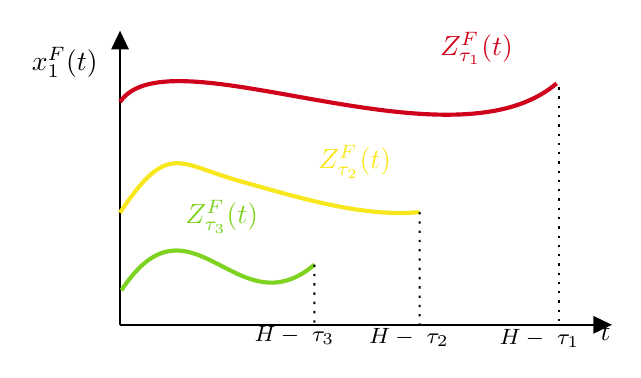
\begin{tikzpicture}[x=0.75pt,y=0.75pt,yscale=-1,xscale=1]
%uncomment if require: \path (0,300); %set diagram left start at 0, and has height of 300

%Straight Lines [id:da2916197270660694] 
\draw    (266,200) -- (500,200) ;
\draw [shift={(503,200)}, rotate = 180] [fill={rgb, 255:red, 0; green, 0; blue, 0 }  ][line width=0.08]  [draw opacity=0] (8.93,-4.29) -- (0,0) -- (8.93,4.29) -- cycle    ;
%Straight Lines [id:da5117089318929615] 
\draw    (266,61.33) -- (266,200) ;
\draw [shift={(266,58.33)}, rotate = 90] [fill={rgb, 255:red, 0; green, 0; blue, 0 }  ][line width=0.08]  [draw opacity=0] (8.93,-4.29) -- (0,0) -- (8.93,4.29) -- cycle    ;
%Curve Lines [id:da7085291191443894] 
\draw [color={rgb, 255:red, 126; green, 211; blue, 33 }   ,draw opacity=1 ][line width=1.5]    (266.67,183.33) .. controls (300.33,132.33) and (322.33,203) .. (359.67,171) ;
%Curve Lines [id:da24493715522522863] 
\draw [color={rgb, 255:red, 248; green, 231; blue, 28 }  ,draw opacity=1 ][line width=1.5]    (266,146) .. controls (288.93,111.26) and (294.39,122.46) .. (322.51,130.39) .. controls (350.62,138.32) and (383.13,148.43) .. (410.33,145.67) ;
%Curve Lines [id:da7705157121253403] 
\draw [color={rgb, 255:red, 208; green, 2; blue, 27 }  ,draw opacity=1 ][line width=1.5]    (266,92.67) .. controls (288.93,57.93) and (425,127.67) .. (476.33,83.67) ;
%Straight Lines [id:da7153614456253439] 
\draw  [dash pattern={on 0.84pt off 2.51pt}]  (477.7,85.5) -- (477.7,200) ;
%Straight Lines [id:da40738299108327425] 
\draw  [dash pattern={on 0.84pt off 2.51pt}]  (410.33,145.67) -- (410.3,200) ;
%Straight Lines [id:da7733686826916204] 
\draw  [dash pattern={on 0.84pt off 2.51pt}]  (359.67,171) -- (359.63,200) ;

% Text Node
\draw (222,64.67) node [anchor=north west][inner sep=0.75pt]    {$x_{1}^{F}( t)$};
% Text Node
\draw (496,197.67) node [anchor=north west][inner sep=0.75pt]    {$t$};
% Text Node
\draw (296,138.67) node [anchor=north west][inner sep=0.75pt]  [color={rgb, 255:red, 126; green, 211; blue, 33 }  ,opacity=1 ]  {$Z_{\tau _{3}}^{F}( t)$};
% Text Node
\draw (360,112) node [anchor=north west][inner sep=0.75pt]  [color={rgb, 255:red, 248; green, 231; blue, 28 }  ,opacity=1 ]  {$Z_{\tau _{2}}^{F}( t)$};
% Text Node
\draw (418.67,57.33) node [anchor=north west][inner sep=0.75pt]  [color={rgb, 255:red, 208; green, 2; blue, 27 } ,opacity=1 ]  {$Z_{\tau _{1}}^{F}( t)$};
% Text Node
\draw (329.33,199.33) node [anchor=north west][inner sep=0.75pt]  [font=\footnotesize]  {$H-\ \tau _{3}$};
% Text Node
\draw (384.5,200) node [anchor=north west][inner sep=0.75pt]  [font=\footnotesize]  {$H-\ \tau _{2}$};
% Text Node
\draw (447.33,200.67) node [anchor=north west][inner sep=0.75pt]  [font=\footnotesize]  {$H-\ \tau _{1}$};


\end{tikzpicture}